\section{Particle analysis}
\label{sec:particle}

In order to understand how the particle converges to the global best, we let $ x^{G} $ be the reference position.
We have interest with three types of movement range, which are defined by three types of reference positions.
\begin{itemize}
\item \textbf{global best} $ \lVert x(k) - x^{G} \rVert $ indicates the distance to the global best, which depends on  $ \lVert x^{P}(k) - x^{G} \rVert $.
\item \textbf{initial position} $ \lVert x(k) - x(0) \rVert $ indicates the distance to the initial position, which depends on $ \lVert x^{G} - x(0) \rVert $ and $ \lVert x^{P}(k) - x(0) \rVert $.
\item \textbf{global optimal} $ \lVert x(k) - x^{*} \rVert $ indicates the distance to the global optimal, which depends on $ \lVert x^{G} -  x^{*} \rVert $ and $ \lVert x^{P}(k) -  x^{*} \rVert $
\end{itemize}

\begin{equation}
\label{eq:rel_gb}
\begin{aligned}
[ v(k+1), x(k+1) - x^{G} ]^{T} = A(k) [ v(k), x(k) - x^{G} ]^{T} + B(k) [ 0, x^{P}(k) - x^{G} ]^{T}
\end{aligned}
\end{equation}
This illustrates that $ \lVert x(k+1) - x^{G} \rVert $ is determined by $ \lVert x^{P}(k) - x^{G} \rVert $.
It also shows that a particle will stop moving when $ x^{P}(k) = x^{G} $.

In order to understand how the boundary of the particle's movement, we let $ x(0) $ be the reference position.
\begin{equation}
\label{eq:rel_init}
\begin{aligned}
[ v(k+1), x(k+1) - x(0) ]^{T} = A(k) [ v(k), x(k) - x(0) ]^{T} + B(k) [ x^{G} - x(0), x^{P}(k) - x(0) ]^{T}
\end{aligned}
\end{equation}
It indicates that $ \lVert x(k+1) - x(0) \rVert  $ is determined by $ \lVert x^{G} - x(0) \rVert $ and $ \lVert x^{P}(k) - x(0) \rVert $.


As in Figure \ref{fig:categorize_regions}, the solution space will be divided into three types of regions by the global best and the personal best.
\begin{itemize}
\item $ f(x) > f(x^G) $
Once a particle gets into this region, it updates both global best and personal best. 
It becomes a leader of the swarm.
\item $ f(x^{G}) > f(x) > f(x^{P}) $
Once a particle gets into this region, it updates only the personal best.
The solution space is then re-divided.
\item $ f(x) < f(x^{P}) $
When a particle is in this region, it only moves as a random walk.
\end{itemize}

\begin{figure}
\centering
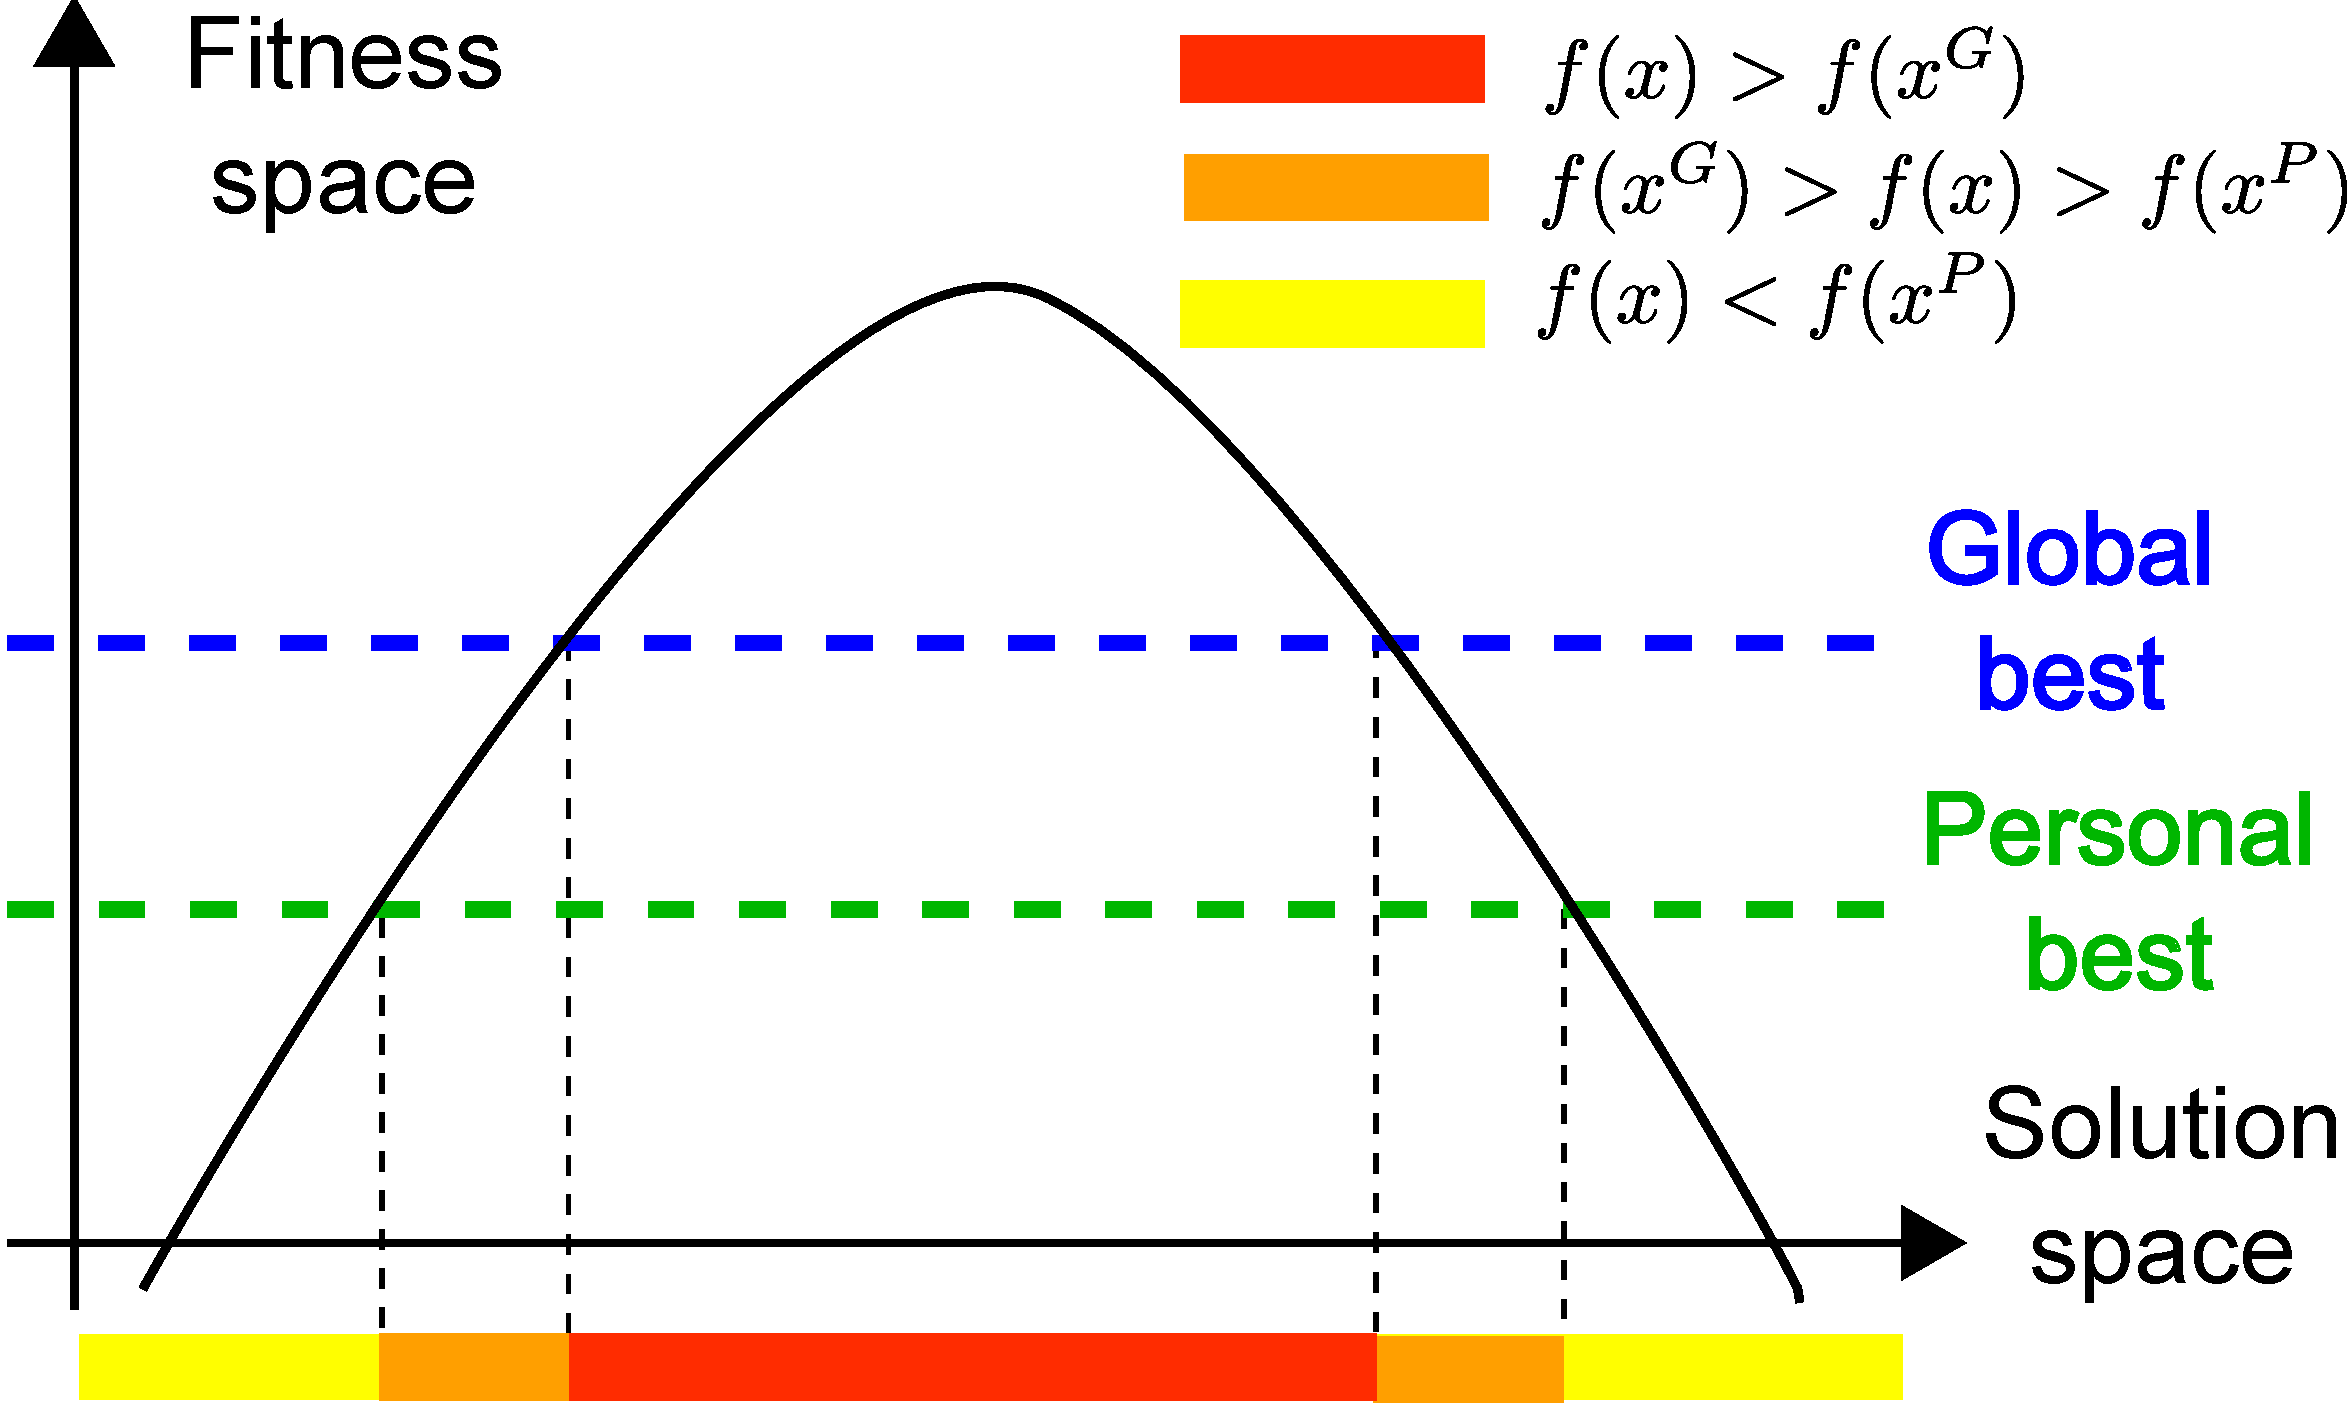
\includegraphics[width=0.7\linewidth]{./fig/categorize_regions}
\caption{How global best and personal best divide the solution space.}
\label{fig:categorize_regions}
\end{figure}

The result of the movement of a particle is determined by which region of the solution space it moves in.

\subsection{What happens in a single hill case}

When the fitness distribution is a single hill, the analysis can be easier.
In most of the cases, the particles should all converge into a single hill where the global best locates in.



It means that there is no effect from a personal best.p
[TODO] random walk reaching a point


\begin{mylem}
In a single hill case, when $ x^{G} = x^{*} $, the particle will converge to $ x^{G} $ if the particle is ISS.
\end{mylem}

\begin{mylem}
In a single hill case, when $ f( x^{G} ) < f( x^{*}) $, the particle will converge to $ \hat{x^{*}} $ and $ f(\hat{x^{*}}) > f(x^{G}) $ if the particle is ISS.
\end{mylem}

\begin{figure}[ht]
\centering
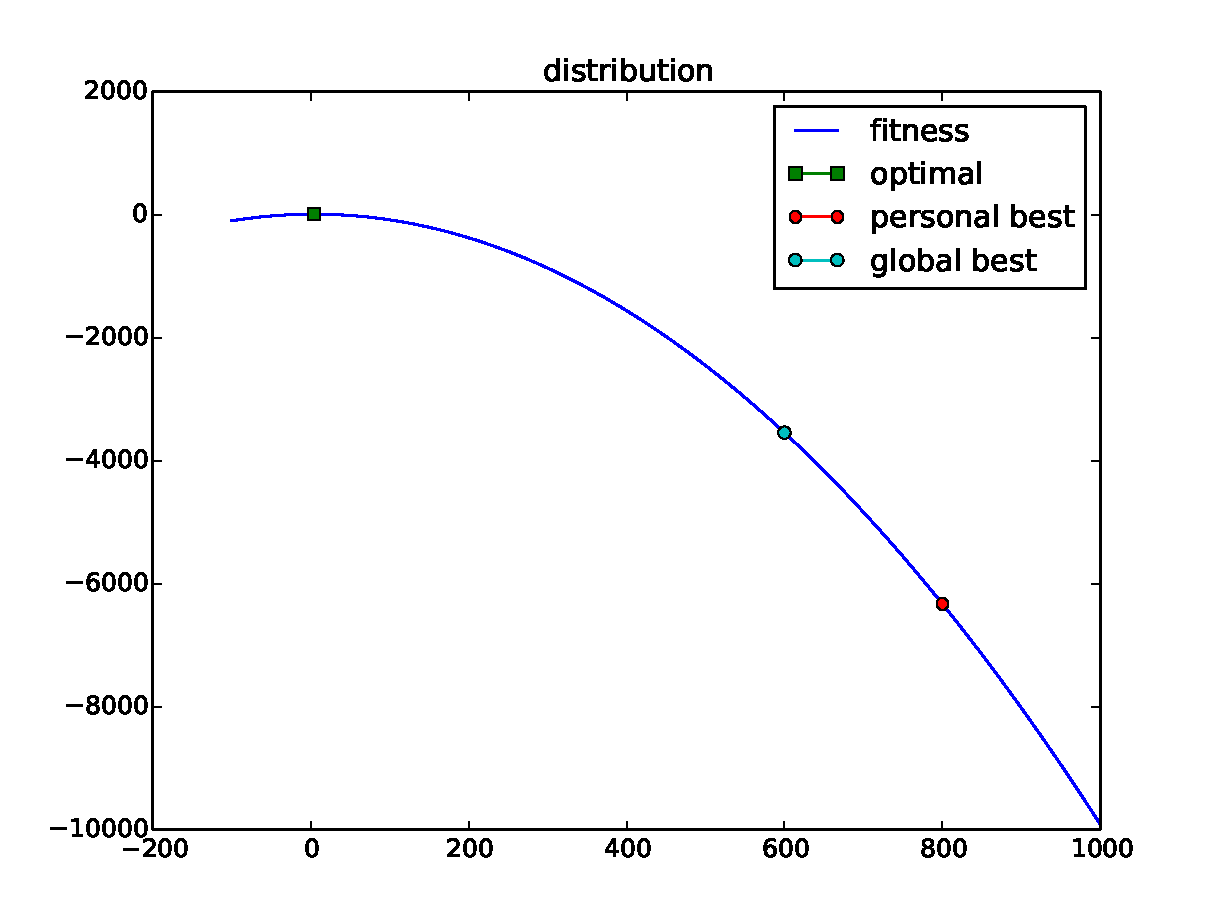
\includegraphics[width=.7\linewidth]{./simfig/case1/distribution1}
\label{fig:case1-1:distribution} 
\end{figure}

\begin{figure}[ht]
\centering
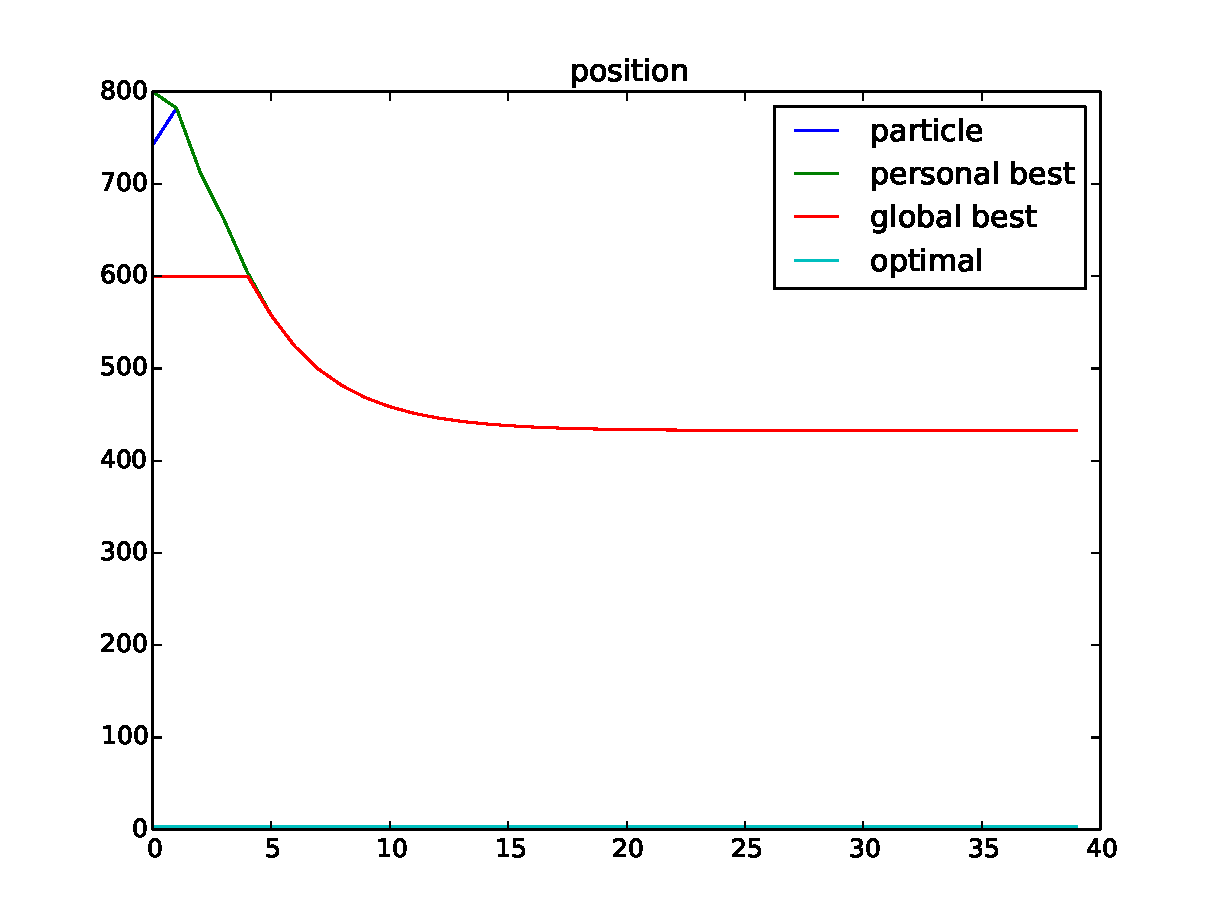
\includegraphics[width=.7\linewidth]{./simfig/case1/position1-1} 
\label{fig:case1-1:position}
\caption{$ \chi = 0.72984 , \phi^{P} = 2.05 , \phi^{G} = 2.05 $ }
\end{figure}

\begin{figure}[ht]
\centering
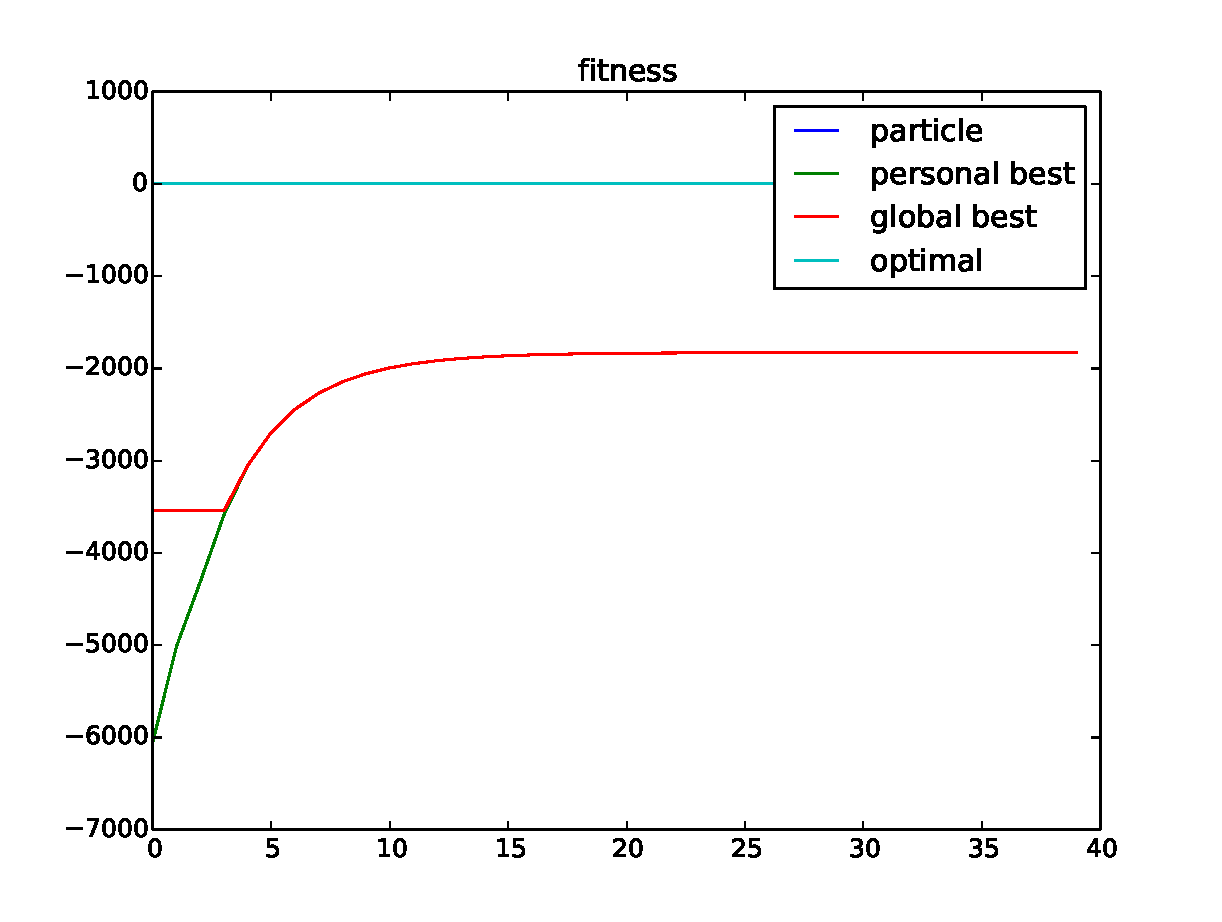
\includegraphics[width=.7\linewidth]{./simfig/case1/fitness1-1} 
\label{fig:case1-1:fitness}
\caption{$ \chi = 0.72984 , \phi^{P} = 2.05 , \phi^{G} = 2.05 $ }
\end{figure}

\begin{figure}[ht]
\centering
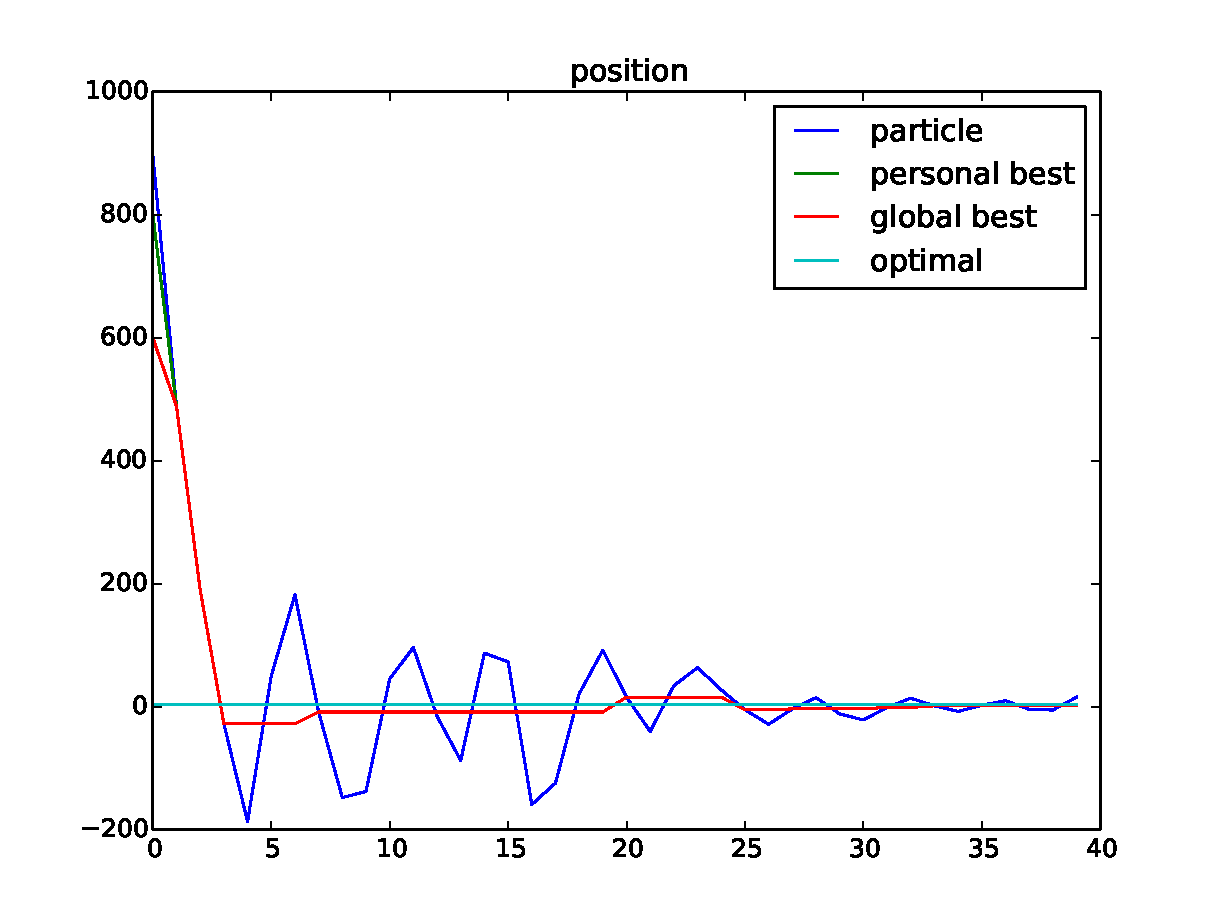
\includegraphics[width=.7\linewidth]{./simfig/case1/position1-2} 
\label{fig:case1-2:position}
\caption{$ \chi = 0.72984 , \phi^{P} = 2.05 , \phi^{G} = 2.05 $ }
\end{figure}
  
\begin{figure}[ht]
\centering
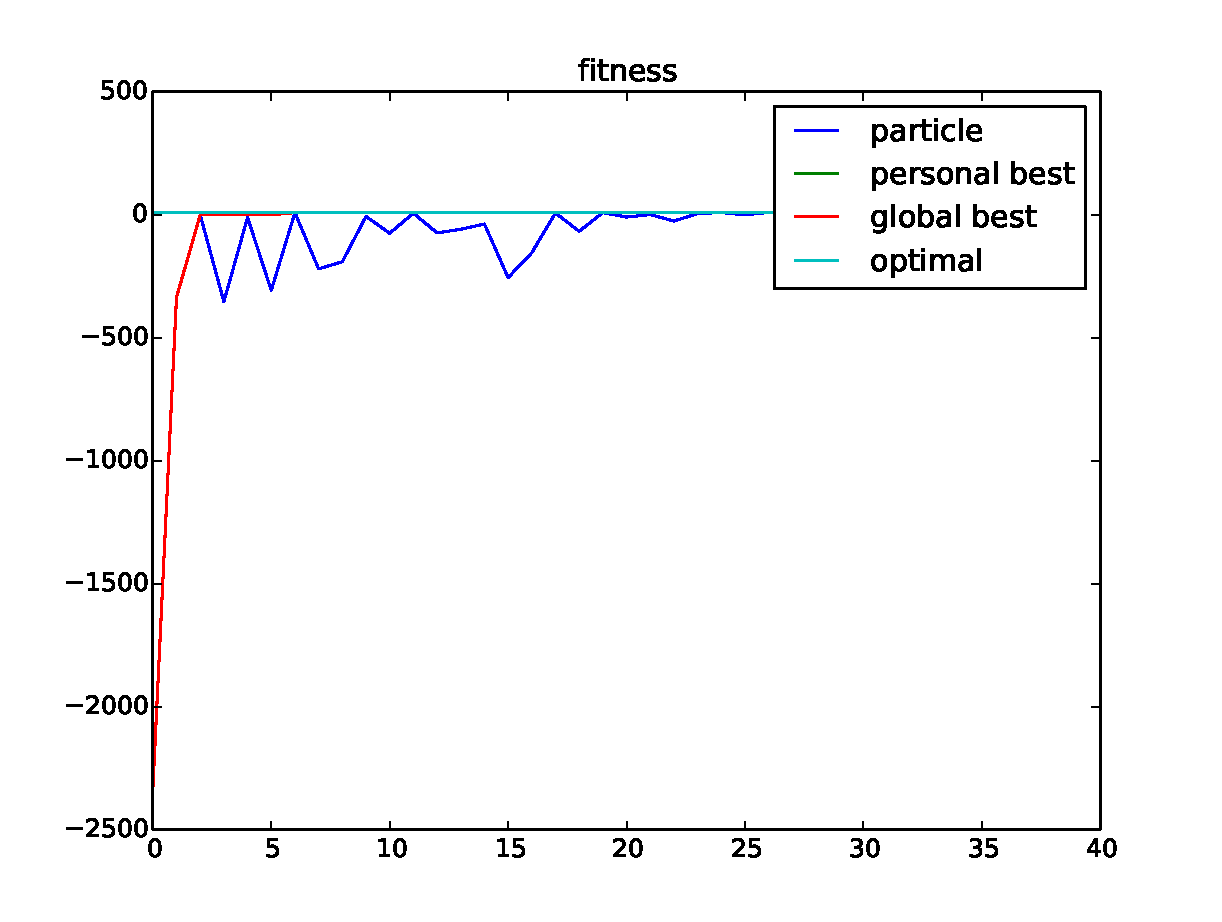
\includegraphics[width=.7\linewidth]{./simfig/case1/fitness1-2} 
\label{fig:case1-2:fitness} 
\caption{$ \chi = 0.72984 , \phi^{P} = 2.05 , \phi^{G} = 2.05 $ }
\end{figure}

Show the exploitation


\subsection{More than single hill case}

Show the exploration

\begin{figure}[ht]
\centering
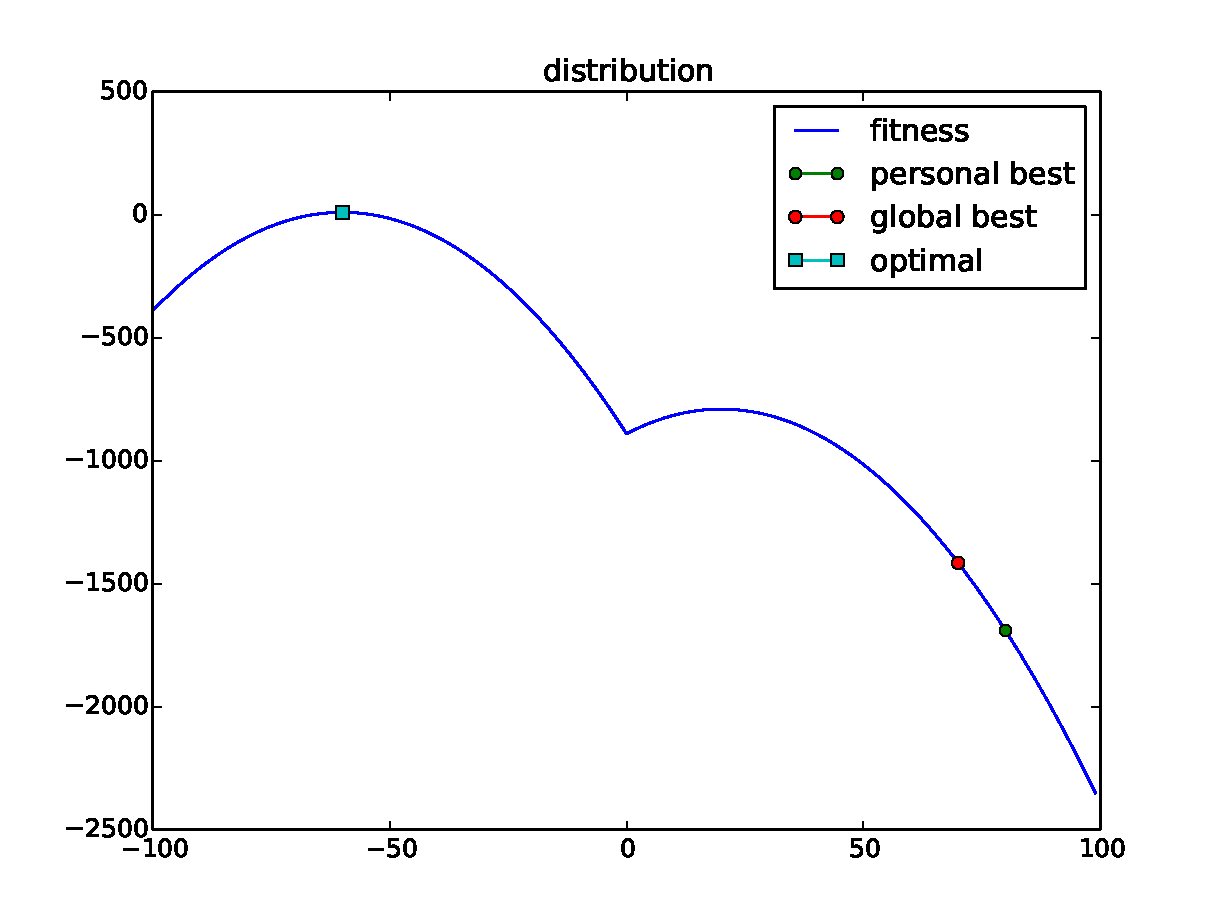
\includegraphics[width=.7\linewidth]{./simfig/case2/distribution2}
\label{fig:case2-1:distribution} 
\end{figure}

\begin{figure}[ht]
\centering
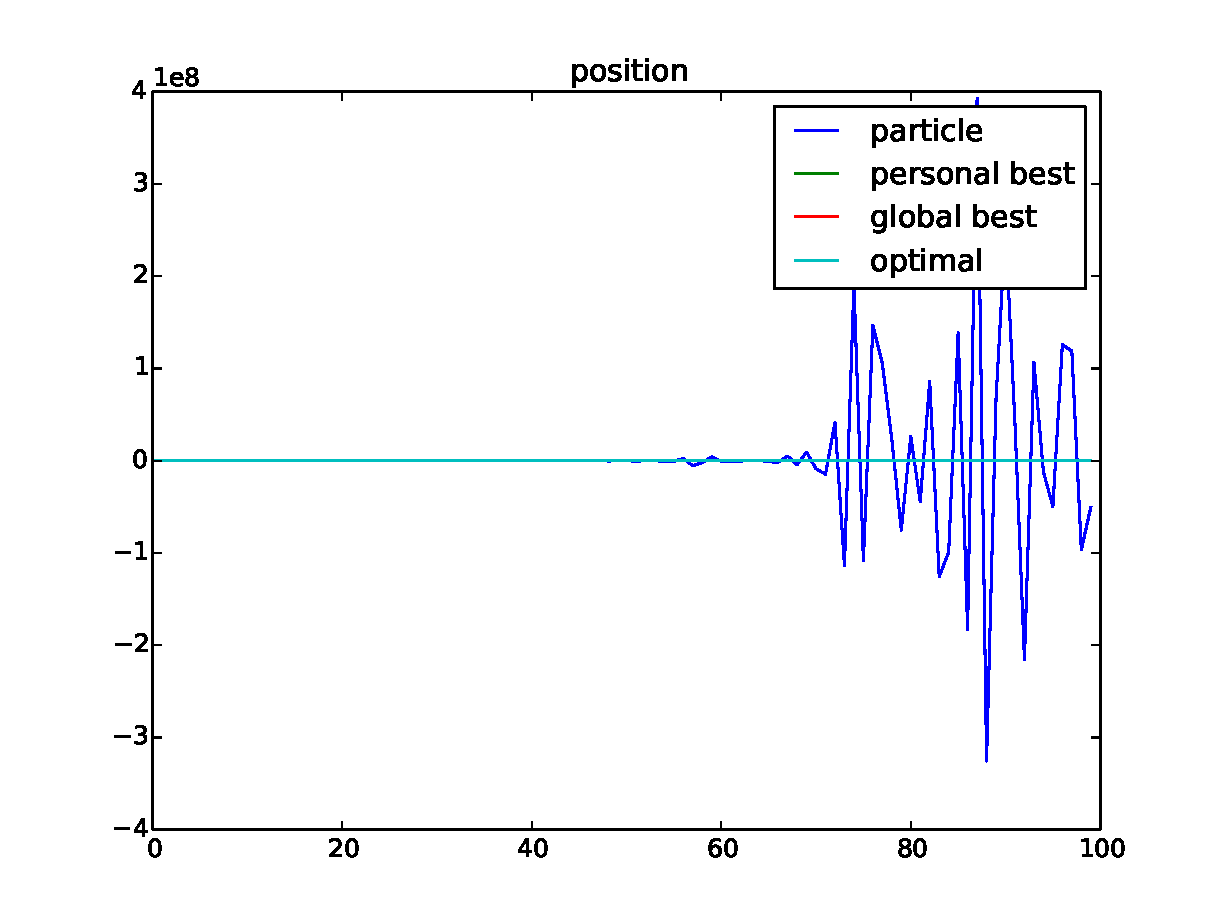
\includegraphics[width=.7\linewidth]{./simfig/case2/position2-1} 
\label{fig:case2-1:position}
\caption{$ \chi = 0.72984 , \phi^{P} = 2.05 , \phi^{G} = 2.05 $ }
\end{figure}

\begin{figure}[ht]
\centering
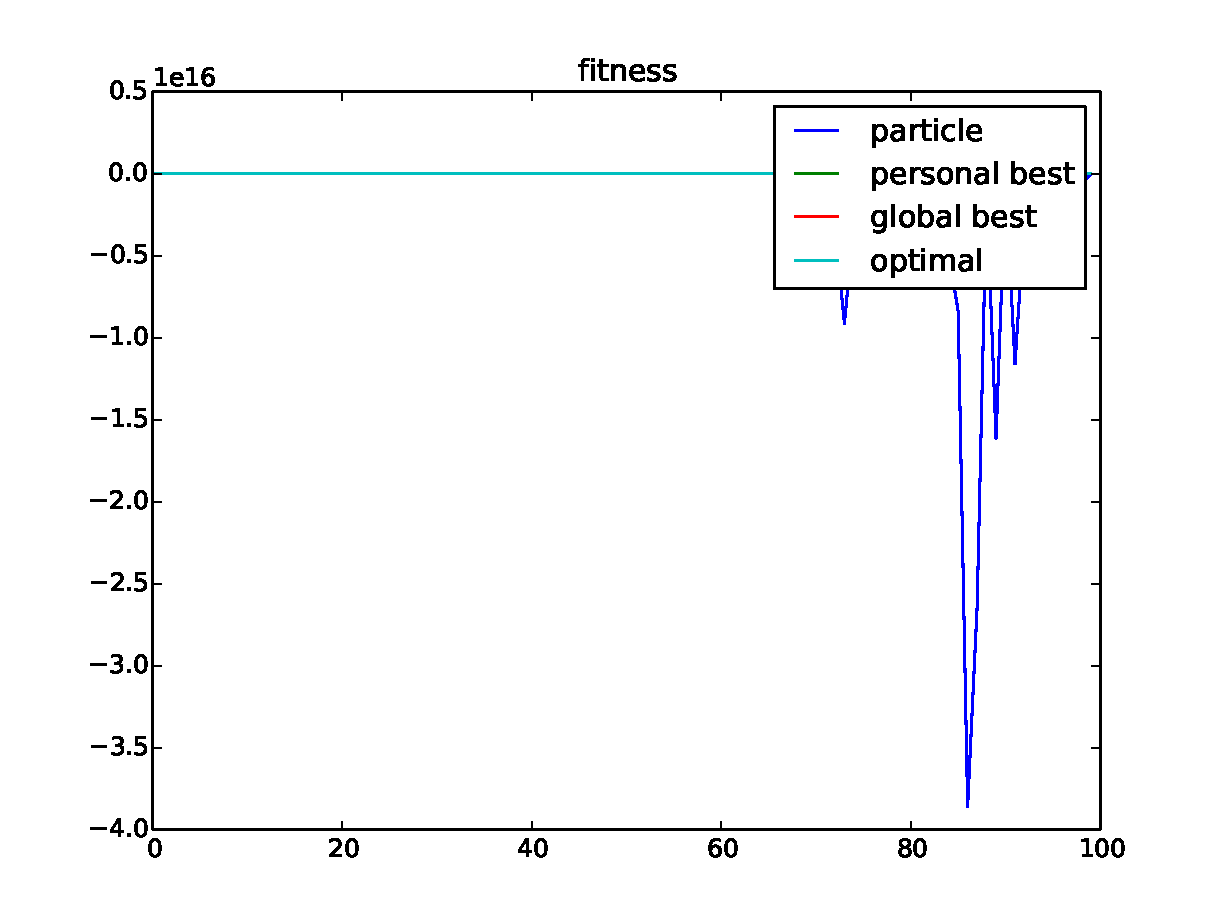
\includegraphics[width=.7\linewidth]{./simfig/case2/fitness2-1} 
\label{fig:case2-1:fitness}
\caption{$ \chi = 0.72984 , \phi^{P} = 2.05 , \phi^{G} = 2.05 $ }
\end{figure}

\begin{figure}[ht]
\centering
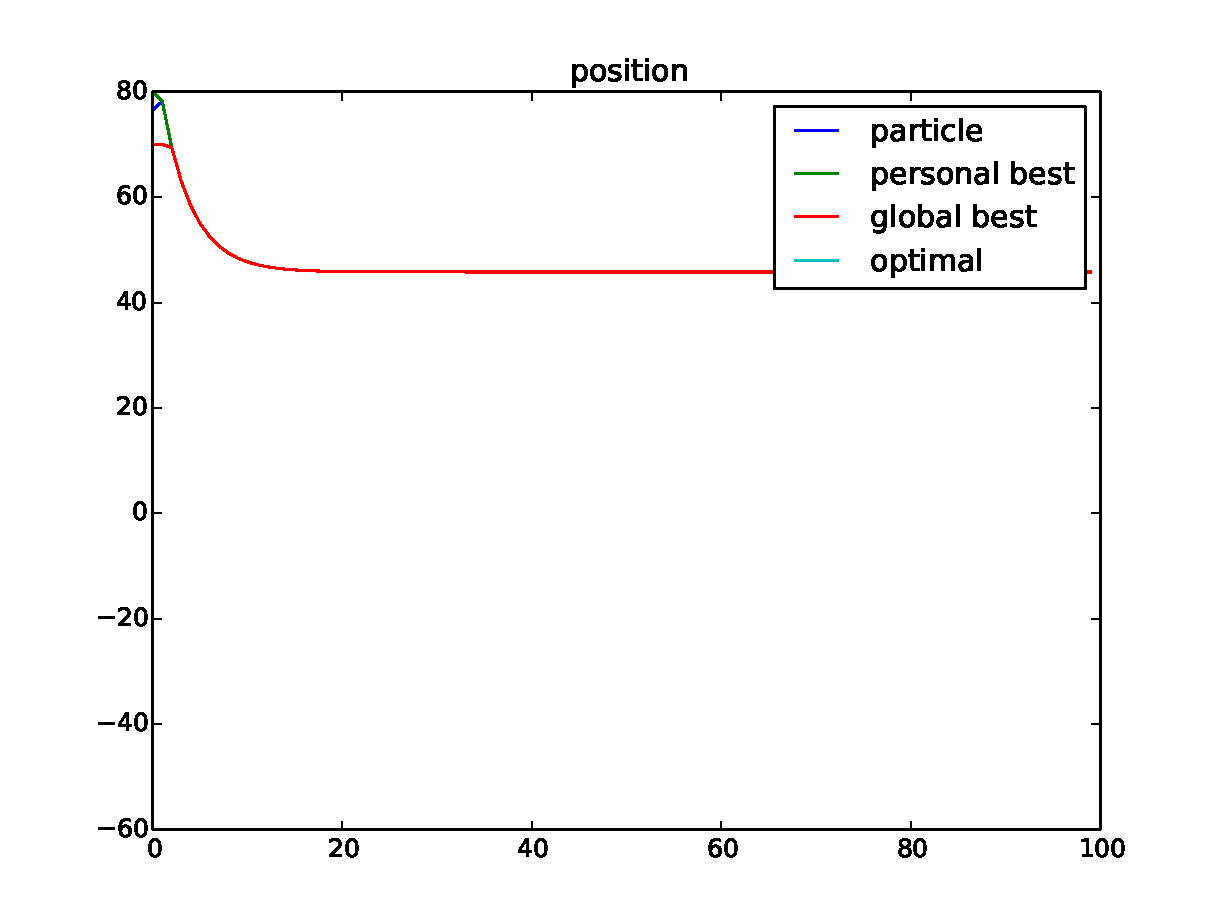
\includegraphics[width=.7\linewidth]{./simfig/case2/position2-2} 
\label{fig:case2-2:position}
\caption{$ \chi = 0.72984 , \phi^{P} = 2.05 , \phi^{G} = 2.05 $ }
\end{figure}
  
\begin{figure}[ht]
\centering
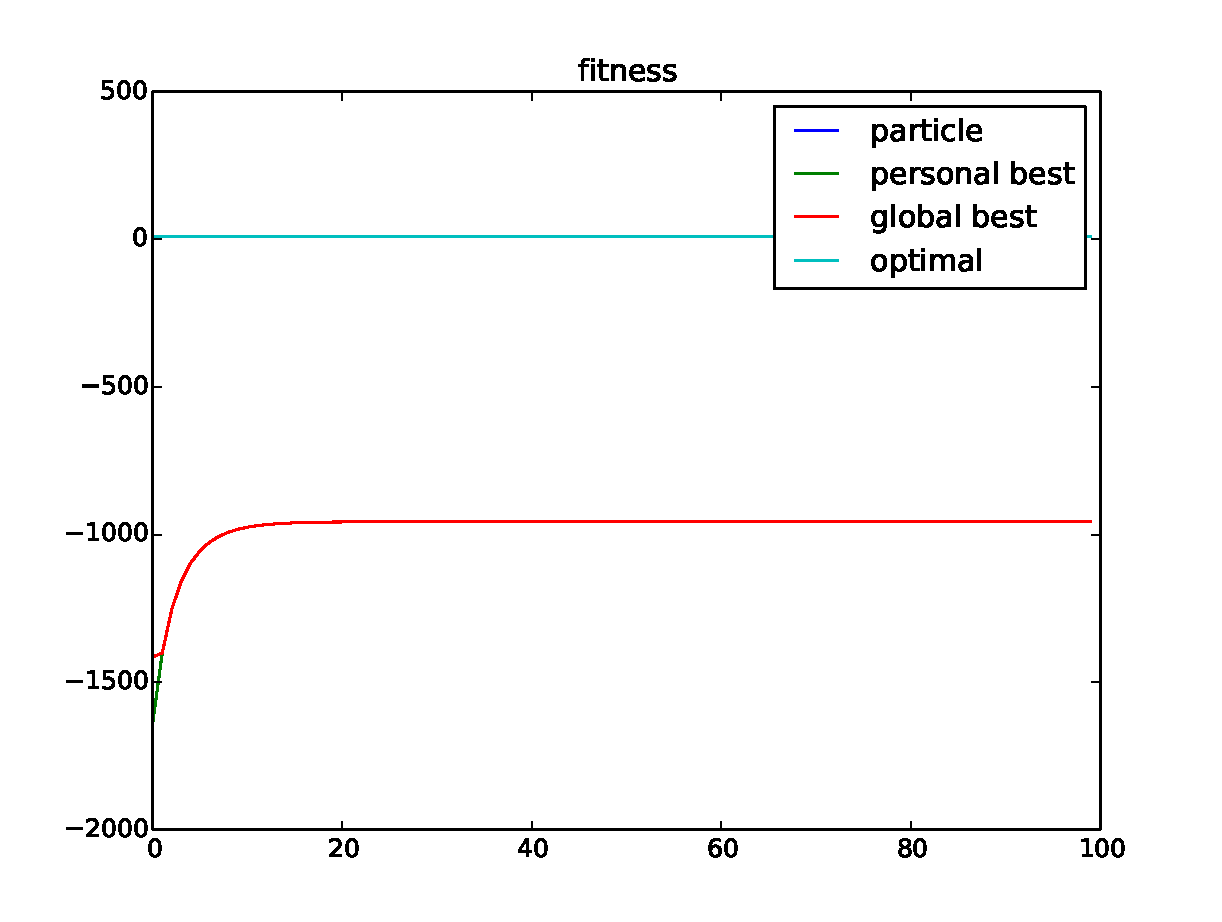
\includegraphics[width=.7\linewidth]{./simfig/case2/fitness2-2} 
\label{fig:case2-2:fitness} 
\caption{$ \chi = 0.72984 , \phi^{P} = 2.05 , \phi^{G} = 2.05 $ }
\end{figure}

